\chapter{Introduction}

\renewcommand{\labelitemi}{$\bullet$}
\section{Problème à résoudre}
L'objectif de ce projet est de réaliser un Global Positioning System «amélioré». Sans entrer dans les détails, un GPS est réalisé à partir d'une modélisation sous forme de graphe orienté d'une carte où les positions sont des nœuds et les routes sont des arcs. L'application d'algorithmes de plus courts chemins sur ces graphes permettent alors de répondre au problème concret du calcul d'itinéraires. Cependant il est rare, dans la vie réelle, que ce type de problème admette une unique contrainte. Ici nous allons travailler sur des graphes plus complexes (voir figure ci-après) par leurs nombres de paramètres
\newline
\newline
\newline
\begin{figure}[!h] 
\begin{center}
  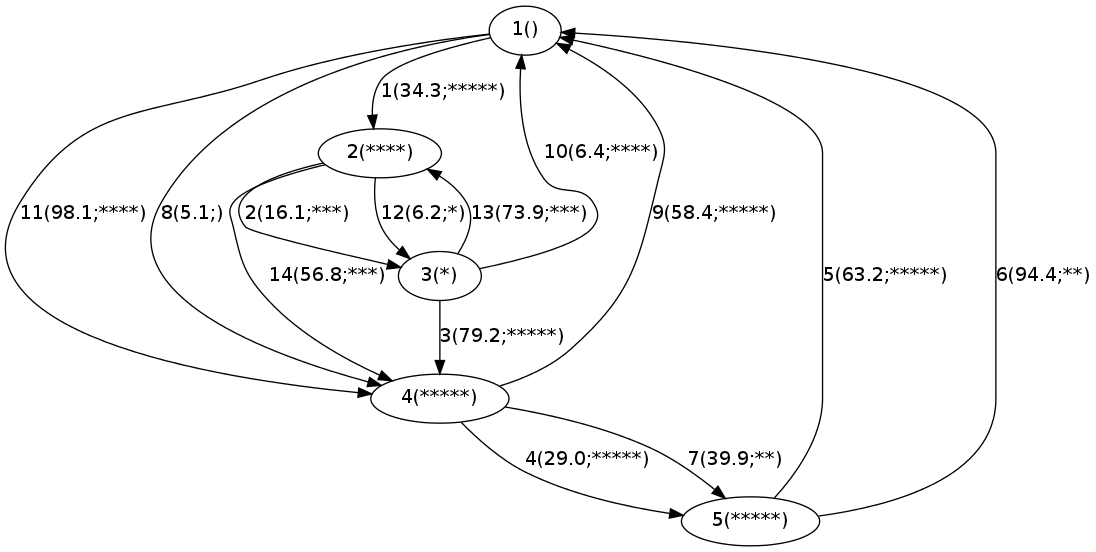
\includegraphics[scale=0.40]{g.png}
\end{center}
\caption{Exemple de graphe étudié}
\end{figure} 


\clearpage


L'idée de réaliser un GPS prenant aussi en compte l'aspect touristique d'un lieu ou d'une route donne les opportunités suivantes : 
\begin{itemize}
\item
Une étude approfondie des algorithmes sur les graphes étudiés en cours pour choisir le plus adapté en fonction du problème et de la structure de données concrète.
\item
Des manipulations plus complexes de ces algorithmes puisque ils prennent plusieurs (et non un seul) paramètres en compte.
\item
Ces différents choix de combinaisons d'implémentations et d'algorithmes entraînes des calculs variés.
\end{itemize}

Tous ces aspects sont au cœur même du module Structures complexes et algorithmique. La première partie du projet se contentait d'étudier et d'implémenter des structures et des algorithmes complexes. Au terme de l'ultime partie, nous réalisons à partir de ces outils  théoriques une application concrète de ces outils abstraits.

\clearpage

\section{Application réalisée}

\subsection{Structure du programme}
Dans la continuité de la première partie du projet, nous avons conçu de nouvelles classes en nous appuyant sur celles de notre graphe orienté. Voici la liste des différents fichiers du package GPS : 

\begin{itemize}
\item
Ville.java : Composée d'un nom et d'une entier qualité dénombrant le nombre d'étoiles
\item
Route.java : Héritant de la classe Arc.java, possède un plus une longueur  et d'une qualité tout comme Ville.java
\item
GPS.java : Comporte les différentes méthodes demandées dans le sujet. Le constructeur prend en compte les données fournies par le parseur ainsi que celle saisie sur l'entrée standards par l'utilisateur
\item
Parser.java : Parse le fichier fourni en paramètre et retourne à la classe appelante le graphe créé ainsi que la distance max entre deux villes sur le graphe, la meilleure qualité, et un annuaire inversé qui donne l'id d'un nœud ou d'un arc dans le graphe à partir de son nom.
\end{itemize}


\subsection{Déroulement de l'application}
Le programme se lance sans paramètres. Il demande à l'utilisateur d'entrer successivement : 
\begin{itemize}
\item
Le nom du fichier d'entrée (devant être présent dans le dossier courant).
\item
Le choix d'implémentation (l la liste d'adjacence et m pour la matrice d'adjacence).
\item
Le nom de la ville de départ.
\item
Le nom de la ville d'arrivée.
\item 
La valeur (K ou A) du paramètre en fonction de la méthode choisie.
\end{itemize}
L'itinéraire calculé sera alors affiché selon les consignes du sujet. Le programme se termine par la suite. Il faut relancer le programme un autre calcul.
 

